%!TEX root=kapfhammer_gcc_presentation.tex
% mainfile: ../kapfhammer_gcc_presentation.tex

\begin{frame}[t]

  \frametitle{Random Testing}
  \framesubtitle{It is easy to randomly generate tests --- but how good are they?}

  \vspace*{.2in}
  \hspace{.4in}
  \resizebox{3.0in}{!}{
    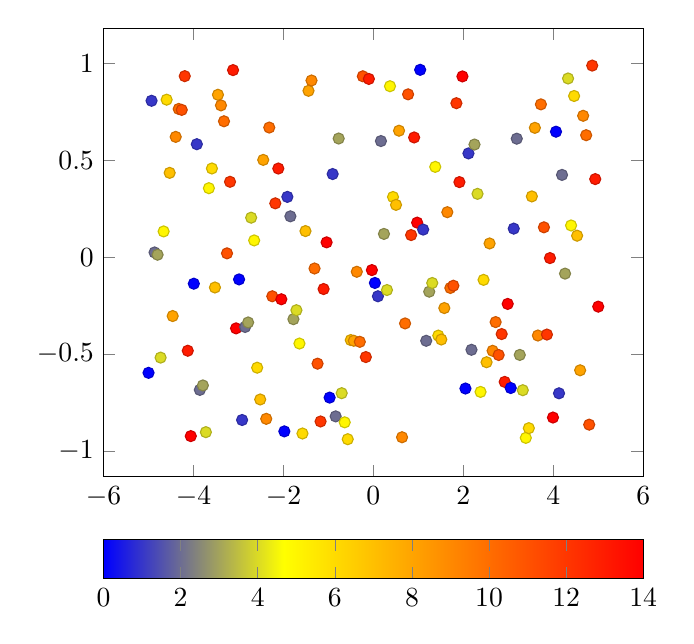
\begin{tikzpicture}
      \begin{axis}[colorbar horizontal]
        \addplot[only marks,scatter,
          scatter src={mod(\coordindex,15)},samples=150]
          {rand};
      \end{axis}
  \end{tikzpicture}}

\end{frame}
